\documentclass{beamer}

% Must be loaded first
\usepackage{tikz}

\usepackage[utf8]{inputenc}
\usepackage{textpos}

% Font configuration
\usepackage{fontspec}

\input{font.tex}

% Tikz for beautiful drawings
\usetikzlibrary{mindmap,backgrounds}
\usetikzlibrary{arrows.meta,arrows}
\usetikzlibrary{shapes.geometric}

% Minted configuration for source code highlighting
\usepackage{minted}
\setminted{highlightcolor=black!5, linenos}
\setminted{style=perldoc}

\usepackage[listings, minted]{tcolorbox}
\tcbset{left=6mm}

% Use the include theme
\usetheme{codecentric}

% Metadata
\title{Dhall: An Introduction}
\author{Markus Hauck @markus1189}

% The presentation content
\begin{document}

\begin{frame}[noframenumbering,plain]
  \begin{center}
    \includegraphics[width=0.5\textwidth]{images/dhall-logo.png}
  \end{center}
  \titlepage{}
\end{frame}

\section{Introduction}\label{sec:introduction}

\begin{frame}
  \frametitle{What Is Dhall}
  \begin{quote}
    A configuration language guaranteed to terminate
  \end{quote}
  \begin{quote}
    dhall is a total programming language specialized to configuration files
  \end{quote}
  \begin{itemize}
  \item from Gabriel Gonzalez (Pipes, Turtle, \ldots{})
  \item language: \url{github.com/dhall-lang/dhall-lang}
  \item haskell: \url{github.com/dhall-lang/dhall-haskell}
  \end{itemize}
 \end{frame}

 \begin{frame}
   \frametitle{Features}
   \begin{itemize}
   \item \textbf{Haskell integration} \textemdash{} Dhall expressions can be
     marshalled into Haskell
   \item \textbf{Total} \textemdash{} Programs always terminate and will never
     hang
   \item \textbf{Safe} \textemdash{} Programs never crash or throw exceptions
   \item \textbf{Distributed} \textemdash{} Expressions can reference other
     expressions by URL or path
   \item \textbf{Strong normalization} \textemdash{} Every expression can be
     reduced to a normal form
   \item \textbf{Statically typed} \textemdash{} Configuration files can be
     validated ahead-of-time
   \item \textbf{Strongly typed} \textemdash{} No coercions, casts or subtyping
   \item \textbf{Built-in data types} \textemdash{} Includes lists, anonymous
     records and anonymous unions
   \end{itemize}
 \end{frame}

 \begin{frame}
   \frametitle{First Example}

   \inputminted{text}{dhall/example-two.dhall}
 \end{frame}

 \begin{frame}
   \frametitle{Useful Tools}
   \begin{itemize}
   \item dhall
   \item dhall-repl
   \item dhall-format
   \item dhall-<json,text,bash>
   \end{itemize}
 \end{frame}

 \section{Dhall Language}

 \begin{frame}
   \frametitle{Language Features}
   \begin{itemize}
   \item Integers
   \item Booleans
   \item Naturals
   \item Strings
   \item Lists
   \item Optionals
   \item Records
   \item \textbf{Unions}
   \item Functions
   \item Imports
   \item Let expressions
   \end{itemize}
 \end{frame}

 \begin{frame}
   \frametitle{Dhall Is Not A General Purpose Language}
   \begin{itemize}
   \item you might get frustrated if you want to program in it
   \item that's not the purpose
   \end{itemize}
 \end{frame}

 \begin{frame}
   \frametitle{Normalization}
   \begin{itemize}
   \item total: every program terminates (eventually)
   \item seems like a heavy restriction
   \item some pretty cool optimizations
   \item reduce/optimize programs with partial input possible
   \item TODO: example
   \end{itemize}
 \end{frame}

 \begin{frame}
   \frametitle{But Why Not XYZ}
   \begin{itemize}
   \item okay no presentation is complete without a rant
   \item JSON
     \begin{itemize}
     \item no comments
     \item repetition
     \item annoying to write
     \item no types!
     \end{itemize}
   \item YAML
     \begin{itemize}
     \item even more awful
     \item think you know YAML?\@ Let's see
     \end{itemize}
   \end{itemize}
 \end{frame}

 \begin{frame}
   \frametitle{JSON for Configuration}
   \begin{center}
     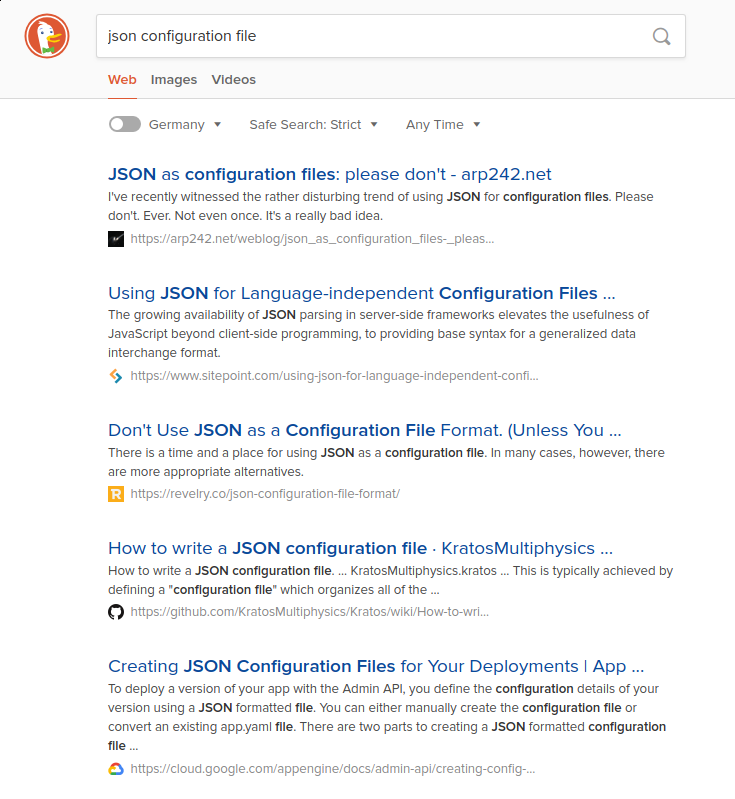
\includegraphics[width=0.6\textwidth]{static-images/duckduckgo-dont-use-json.png}
   \end{center}
 \end{frame}

 \begin{frame}
   \frametitle{Unions}
   \begin{itemize}
   \item the constructors keyword
   \item smart constructors
   \item mapping to Haskell
   \end{itemize}
 \end{frame}

 \begin{frame}
   \frametitle{Imports}
   \begin{itemize}
   \item file imports
   \item url imports
   \item
   \end{itemize}
 \end{frame}

 \begin{frame}
   \frametitle{The Prelude}
   \begin{itemize}
   \item List
   \item Optional
   \end{itemize}
 \end{frame}

 \begin{frame}
   \frametitle{Mapping To Haskell}
 \end{frame}

 \section{Getting Out}

 \begin{frame}
   \frametitle{To JSON}
   % https://github.com/dhall-lang/dhall-json
 \end{frame}

 \begin{frame}
   \frametitle{To YAML}
 \end{frame}

 \begin{frame}
   \frametitle{To Bash}
   % https://github.com/dhall-lang/dhall-bash
 \end{frame}

 \begin{frame}
   \frametitle{To Text}
   % https://github.com/dhall-lang/dhall-text
 \end{frame}

 \begin{frame}
   \frametitle{To Nix}
   % https://github.com/dhall-lang/dhall-nix
 \end{frame}

 \begin{frame}
   \frametitle{To Cabal}
   % https://github.com/dhall-lang/dhall-to-cabal
 \end{frame}

 \begin{frame}
   \frametitle{To K8s}
   % https://github.com/dhall-lang/dhall-kubernetes
 \end{frame}

 \section{Conclusion}

 \begin{frame}
   \frametitle{References}
   \begin{itemize}
   \item language: \url{github.com/dhall-lang/dhall-lang}
   \item haskell: \url{github.com/dhall-lang/dhall-haskell}
   \item tutorial: \url{hackage.haskell.org/package/dhall/docs/Dhall-Tutorial.html}
   \end{itemize}
 \end{frame}

\appendix{}

\section*{Bonus}\label{sec:bonus}

\end{document}
